\documentclass{VUMIFPSmagistrinis}
\usepackage{algorithmicx}
\usepackage{algorithm}
\usepackage{algpseudocode}
\usepackage{amsfonts}
\usepackage{amsmath}
\usepackage{bm}
\usepackage{caption}
\usepackage{color}
\usepackage{float}
\usepackage{graphicx}
\usepackage{listings}
\usepackage{subfig}
\usepackage{wrapfig}
\usepackage[table,xcdraw]{xcolor}

\newcolumntype{L}{>{\columncolor{black}\color{white}}l}


\university{Vilniaus universitetas}
\faculty{Matematikos ir informatikos fakultetas}
\department{Informatikos institutas}
\papertype{Programų sistemų architektūros ir projektavimo laboratorinis darbas}
\title{Architektūriniai požiūriai}
\titleineng{Architectural viewpoints}
\author{Matas Savickis}
\reviewer{}

\supervisor{Rimantas Kybartas, Partn. Prof., Dr.}

\date{Vilnius – \the\year}

\bibliography{bibliografija}

\begin{document}
\maketitle

\tableofcontents
	\section{Sistema}
		Žmonės turi daiktų, kuriuos nori parduoti, tačiau nežino kiek tiksliai jų parduodamas daiktas gali būti vertas.
		Sistema leidžia vartotojams parduoti daiktus aukciono principu.
		Vartotojas įdeda norimą daiktą į aukcioną nustatydamas mažiausią kainą už kurią sutiktų parduoti daiktą, nustato aukciono trukmę ir kiti sistemos parduotojai gali didinti daikto kainą iki nustatyto laiko.
		Sistema suteikia galimybę atsiskaityti už prekes elektroninio banko pervedimais ir kriptovaliutomis.
	\section{Suinteresuoti asmenys}
		\begin{itemize}
			\item{Pirkėjai - vartotojai, kurie naudosis aukcionu siekdami parduoti prekę.}
			\item{Pardavėjai - vartotojai, kurie naudosis aukcionu siekdami nusipirkti prekę.}
			\item{Investuotojai - žmonės, kurie rems projekto įgyvendinimą finansiškai}
			\item{Programuotojai - žmonės, kurie kurs sistemą.}
			\item{Testuotojai - žmonės, kurie testuos sistemą.}
			\item{Policija - suinteresuota nelegalių daiktų pirkėjų ir pardavėjų identifikavimu.}
			\item{Lietuvos teismas - suinteresuotas nelegalių prekių pirkimu ir pardavimu, taip pat Lietuvos įstatymų laikymusi.}
			\item{Europos sąjunga - suinteresuota, kad sistema laikytusi europos sąjungos įstatymų ir reglamentų(BDAR)}
		\end{itemize}
		\section{Konteksto požiūrio taškas}
			\subsection{Sistemos taikymo sritis}
				Vartotojas sistemoje įkelią savo skelbimą, kiti vartotojai dalyvauja aukcione ir didžiausią kainą pasiūlęs vartotojas laimi aukcioną.
				Aukcioną laimėjęs žmogus perveda pinigus arba Bitcoin kripto valiutą į mūsų sistema, tuomet prekės pardavėjas išsiunčia prekę į mūsų biurą patikrinti ar prekė atitinka aprašymą. 
				Biuro darbuotojui patvirtinus, kad prekė atitinka aprašymą sistema perveda pinigus pardavėjui jo pasirinktu būdu.

			\subsection{Konteksto požiūrio taško diagrama}

				\begin{figure}[H]
				\centering
				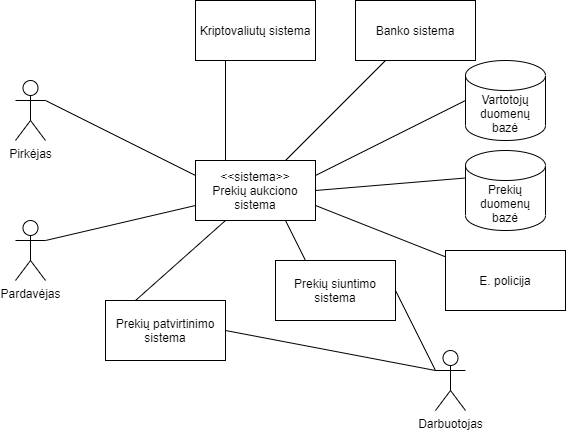
\includegraphics[scale=0.9]{img/context}
				\caption{Aukciono sistemos konteksto požiūrio taško diagrama} % Antraštė įterpiama po paveikslėlio
				\label{img:text}
				\end{figure}
	
			\subsection{Funkciniai reikalavimai}
				\subsubsection{Pardavėjas reikalavimai}
					\begin{enumerate}
						\item{Pirkėjas turi galimybę įdėti prekę į aukcioną nurodydamas jos pradinę kainą, aukciono trukmę, aprašymą ir įkeldamas fotogtafiją.}
						\item{Pirkėjas atšaukti aukcioną jam nepasibaigus taip nebeparduodant prekės.}
						\item{Atsiradus pirkėjui, po aukciono pardavėjas turi prekę išsiųsti į aukciono sandelį per dvi darbo dienas.}
						\item{Pirkėjas pardavęs prekę gali pasirinkti išmokėjimo būdą: pavedimas į sąskaitą, kriptovaliutas, aukciono sąskaitos papildymas.}
					\end{enumerate}
				\subsubsection{Pirkėjas reikalavimai}
					\begin{enumerate}
						\item{Pirkėjas norėdamas dalyvauti aukcione turi įsidėti pinigų į aukciono sąskaitą.}
						\item{Aukciono sąskaitą galima papildyti per elektroninį banką arba pervedant kripto valiutas į sistemos piniginę.}
						\item{Pirkėjas gali siūlyti didesnę prekės kainą kol prekės aukcionas nepasibaigė.}
						\item{Paskutinis aukščiausią kainą pasiūlęs pirkėjas laimi aukcioną.}
						\item{Aukciono nugalėtojas gali sekti jam atkeliaujančia prekę.}
						\item{Nugalėtojui negavus prekės jo pinigai pervedami į aukciono sąskaitą.}
						\item{Pirkėjas gali komentuoti prie kiekvienos prekės.}
						\item{Pirkėjas gali persivesti savo aukciono sąskaitą į savo kriptovaliutų piniginę arba į savo bankinę sąskaitą.}
					\end{enumerate}
				\subsubsection{Prekių siuntimo reikalavimai}
					\begin{enumerate}
						\item{Pardavėjui atsiuntus prekę į aukciono sandėlį prekė yra patvirtinama aukciono darbuotojo ar siuntinys atitinka aukcione pateiktą prekės aprašymą ir nuotrauką.}
						\item{Gavus įtartiną siuntinį aukciono darbuotojas informuoja policiją pateikdamas pirkėjo ir pardavėjo duomenis}
						\item{Jeigu prekė neatitinka aprašymo ir fotografijos pinigai būna gražinami pirkėjui ir krepė yra išsiunčiama pardavėjui išperkamosios siuntos principu.}
					\end{enumerate}
				\subsubsection{Banko reikalavimai}
					\begin{enumerate}
						\item{Sistemoje yra galimybė pervesti pinigus iš banko sąskaitos į aukciono sąskaitą.}
						\item{Sistemoje yra galimybę gauti pinigus iš aukciono sąskaitos į banko sąskaitą.}
						\item{Bankinės pranzakcijos yra vykdomos banklink paslauga.}
					\end{enumerate}
				\subsubsection{Kriptovaliutų reikalavimai}
					\begin{enumerate}
						\item{Sistemoje yra galimybė pervesti kritovaliutas iš kripto piniginės į aukciono sąskaitą, kripto valiutos automatiškai konvertuojamos į eurus taikant papildoma mokestį. }
						\item{Sistemoje yra galimybė pervesti pinigus iš aukciono sąskaitos į kriptovaliutų piniginę taikant papildomą mokestį.}
					\end{enumerate}
				\subsubsection{Policijos reikalavimai}
					\begin{enumerate}
						\item{Policijai apie nelegalias prekes yra pranešama naudojanti e. Policija paslaugomis.}
					\end{enumerate}
				\subsubsection{Teisiniai reikalavimai}
					\begin{enumerate}
						\item{Sistema veikia laikydamasi Lietuvos įstatymų.}
						\item{Sistema veikia laikydamasi Europos įstatymų ir BDAR reglamento.}
					\end{enumerate}
				\subsubsection{Bendri reikalavimai}
					\begin{enumerate}
						\item{Vartotojui paprašius jo duomenys yra pašalinami iš sistemos per mėnesį.}
						\item{Vartotojas gali matyti savo pirkimų ir pardavimų istoriją.}	
					\end{enumerate}
			
		\section{Funkcinis požiūrio taškas}
			Sistema kuriama bandant išlaikyti komponentų atskirtį, sustojus veikti vienam sistemos komponentui, kiti komponentai neturi būti įtakojami.
			Sustojus ,,Prekių aukciono sistema" komponento veikimui vis dar veikia ,,Administravimo sistema" komponento veikimas ir taip toliau.
			\subsection{Komponentų diagrama}
				\begin{figure}[H]
				\centering
				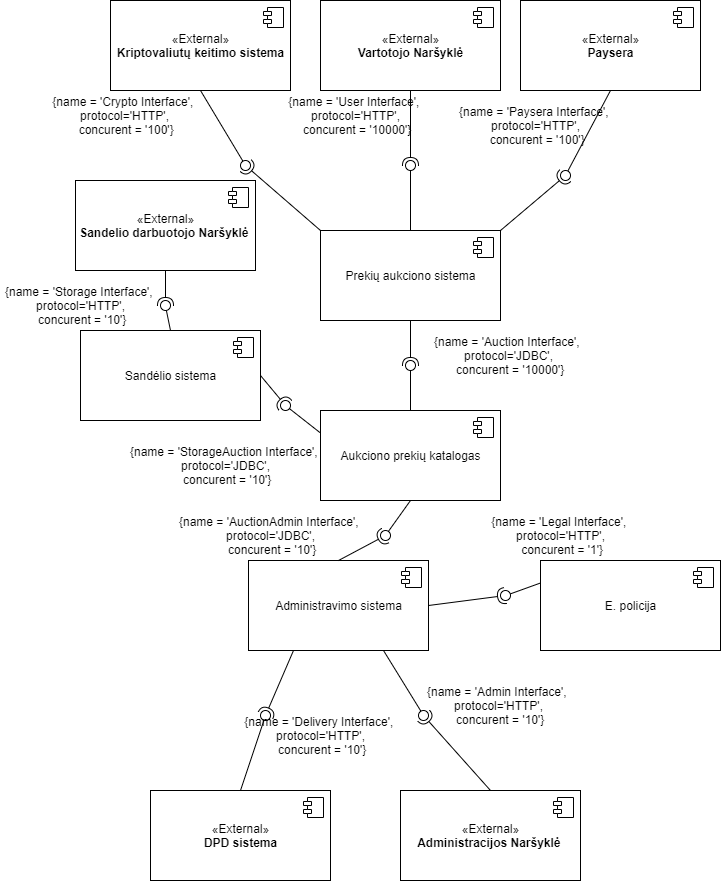
\includegraphics[scale=0.7]{img/function}
				\caption{Kompnentų diagrama} % Antraštė įterpiama po paveikslėlio
				\label{img:text}
				\end{figure}
			\subsection{Interfeisų aprašai}

				\begin{table}[H]
				\centering
				\begin{tabular}{|L|p{9cm}|}\hline
			 		Interfeiso pavadinimas& Crypto Interface\\ \hline
			 		Aprašymas& Interfeisas atsakingas už vartotojų kripto valiutų pervedimus ir pinigų išgryninimą iš kripto valiutos į eurus \\ \hline
				\end{tabular}
				\caption{Crypto Interface}
				\end{table}

				\begin{table}[H]
				\centering
				\begin{tabular}{|L|p{9cm}|}\hline
			 		Interfeiso pavadinimas& User Interface\\ \hline
			 		Aprašymas& Interfeisas skirtas perduoti perduoti duomenis vartotojo naršyklei. Perduodami su aukcionu susije duomenys.  \\ \hline
				\end{tabular}
				\caption{User Interface}
				\end{table}

				\begin{table}[H]
				\centering
				\begin{tabular}{|L|p{9cm}|}\hline
			 		Interfeiso pavadinimas& Paysera Interface\\ \hline
			 		Aprašymas& Skirta atlikti pavedimus pridedant pinigus į aukciono sąskaitą arba juos bandant išsiimti. Šis intefeisas taip pat skirtas pinigus pervesti į įmonės sąskaitą \\ \hline
				\end{tabular}
				\caption{Paysera Interface}
				\end{table}

				\begin{table}[H]
				\centering
				\begin{tabular}{|L|p{9cm}|}\hline
			 		Interfeiso pavadinimas&Storage Interface\\ \hline
			 		Aprašymas&  Šio interfeisu naudojamasi perduoti duomenis sandelio darbuotojo naršyklei bei sandelio daruotojui pranešti apie blogas arba neatitinkančias prekes \\ \hline
				\end{tabular}
				\caption{Storage Interface}
				\end{table}

				\begin{table}[H]
				\centering
				\begin{tabular}{|L|p{9cm}|}\hline
			 		Interfeiso pavadinimas& StorageAuction Interface \\ \hline
			 		Aprašymas&Interfeisas skirtas komunikuoti su aukciono prekiu duomenu baze  \\ \hline
				\end{tabular}
				\caption{ StorageAuction Interface}
				\end{table}

				\begin{table}[H]
				\centering
				\begin{tabular}{|L|p{9cm}|}\hline
			 		Interfeiso pavadinimas& Auction Interface\\ \hline
			 		Aprašymas& Interfeisas skirtas komunikuoti su duomenų baze. Šioje vietoje aukcione atlikti pirkimai ir pardavimai užregistruojami duomenų bazėje. \\ \hline
				\end{tabular}
				\caption{ Auction Interface}
				\end{table}

				\begin{table}[H]
				\centering
				\begin{tabular}{|L|p{9cm}|}\hline
			 		Interfeiso pavadinimas& AuctionAdmin Interface\\ \hline
			 		Aprašymas& Administratoriaus sąsajos bendravimo su aukciono duomenų baze. Čia administratorius gali matyti aukciono informaciją ir ją dalinai koreguoti \\ \hline
				\end{tabular}
				\caption{AuctionAdmin Interface}
				\end{table}

				\begin{table}[H]
				\centering
				\begin{tabular}{|L|p{9cm}|}\hline
			 		Interfeiso pavadinimas& Legal Interface\\ \hline
			 		Aprašymas& Šiame interfese administratorius perduoda reikalingą informacija e.Policijai apie nelegalias prekes siunčiamas aukcione \\ \hline
				\end{tabular}
				\caption{Legal Interface}
				\end{table}

				\begin{table}[H]
				\centering
				\begin{tabular}{|L|p{9cm}|}\hline
			 		Interfeiso pavadinimas& Admin Interface\\ \hline
			 		Aprašymas& Interfeisas per kuri administratorius pasiekią aukciono platformą per naršyklę \\ \hline
				\end{tabular}
				\caption{Admin Interface}
				\end{table}

				\begin{table}[H]
				\centering
				\begin{tabular}{|L|p{9cm}|}\hline
			 		Interfeiso pavadinimas& Delivery Interface\\ \hline
			 		Aprašymas& Interfeisas skirtas administracijai komunikuoti su pristatymu įmone DPD, atlikti siuntų paėmimą ir sekimą. \\ \hline
				\end{tabular}
				\caption{Delivery Interface}
				\end{table}
			\subsection{Procesai apimantys visą sistemą}
				Sistemoje vykdomas įvykių žurnalizavimas sekti vartotojo veiksus sistemoje ir registruoti sistemines klaidas.
				Šis procesas apima visus vidinius sistemos komponentus.
				Žurnalai saugomi sistemos serveryje.
		\section{Diegimo požiūrio taškas}
			Sistema yra išskirstyta į tris skirtingas produkcines aplinkas iš kurių kiekviena aplinka gali būti sukurta kelis kartus siekiant horizontalaus scale'inimo.
			Aplinkoje taip pat yra duomenų bazės mazgas, jo taip pat galima sukurti kelis mazgus siekiant paskirstyti apkrovas.
			Duomenu bazė tampa eventualy consistant.
			Produkcinėje aplinkoje yra backend jar failas, ir front end failai.
			Visos aplinkos veikia ant Linux operacinės sistemos o visi mazgai yra Docker aplinkoje.
			\subsection{Diegimo diagrama}
				\begin{figure}[H]
				\centering
				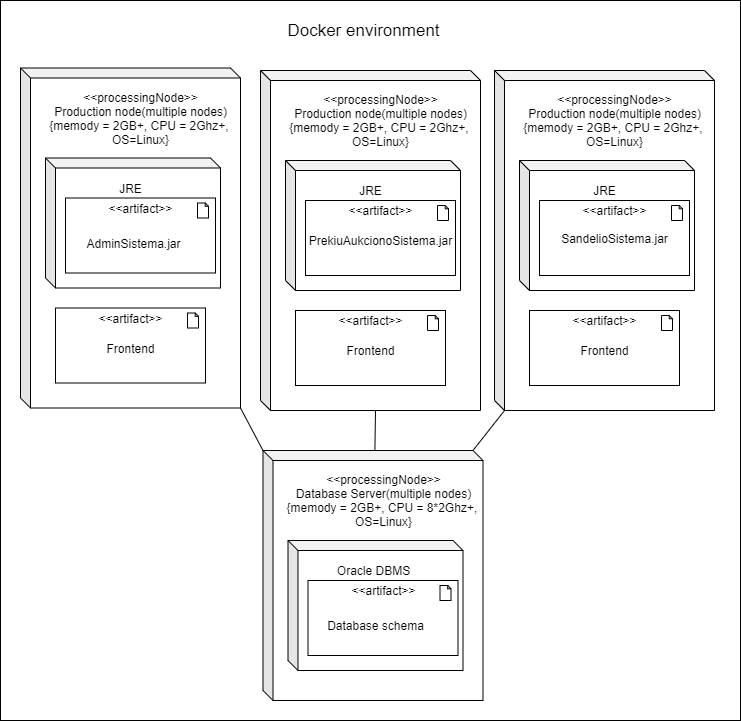
\includegraphics[scale=0.7]{img/deployment}
				\caption{Kompnentų diagrama} % Antraštė įterpiama po paveikslėlio
				\label{img:text}
				\end{figure}
			\subsection{Priklausomybių modelis}
				\begin{itemize}
					\item{JRE 1,8}
					\item{Orable DBMS 11}
					\item{Linux}
					\item{Node.js}
					\item{Spring Boot}
					\item{Docker}
				\end{itemize}
			
		\section{Operatyvinis požiūrio taškas}
			\subsection{Diegimas ir migracija}
				Diegimas vykdomas sukuriant atitinkamus mazgus debesijos aplinkoje.
				Norint paleisti produkcijos Java projektus komandinėje eilutėje reikia įrašyti mvn clean install -Pbuild
				Sistemos modulių veresijos kėlimui naudojama sudo apt-get install.
				
			\subsection{Configūracijos valdymas}
				Vidurnakti yra sukuriamas naujas žurnalizavimo failas sekti sekančios dienos įvykiams ir sisteminėms klaidoms.
				Vidurnakti atliekamas naujos versijos diegimas arba modulių bei bibliotekų update'inimas
			\subsection{Sistemos administravimas}
				Sistemą prižiūri vienas Fullstack programuotojas
		\section{Saugumo perspektyva}
			\subsection{Konteksto požiūrio taško saugumo perspetyva}
				Išoriniai ryšiai ir su jai susijusios grėsmės
				\begin{itemize}
					\item{Vartotojo sąsaja -- į per vartotojo sąsaja gali prisijungti neautorizuotas vartotojas ir gauti vartotojo asmeninius duomenis bei siuntų pristatymo ir išsiuntimo adresus. Susiekti su administracija, kad būtų pakeičiamas siuntos adresas. }
					\item{Kriptovaliutos sistemos sąsaja -- nekorektiškai siunčiant duomenis gali būti perimti ir kripto valiutos persiunčiamos į kitą piniginę}
					\item{Banko sistemos sąsaja -- gresmė panaši kaip ir su kripto valiutomis, nekorektiškai siunčiant duomenis juos būtų galima perimti ir pinigai būtų siunčiami į kitą sąskaitą.}
					\item{Vartotojo duomenų bazė -- gavus administratoriaus lygio prieeigą prie duomenų bazės būtų galima gauti visus asmeninius duomenis saugomus joje.}
					\item{Prekių duomenų bazė -- panašiai kaip ir su vartotojo duomenų bazėmis gavus prieeiga būtų galima gauti duomenis apie siuntas ir taikant socialinės inžinerijos atakas perimtas tas siuntas ir pakeisti adresatus.}
					\item{E. policijos duomenų bazė -- kenkėjiškai sistemai imitavus E. policijos sąsaja būtų galima perimti informaciją apie vartotojus bei paprašyti nelegalių siuntų atsiėmimo.}
					\item{Prekių siuntimo sistemos sąsaja -- gavus prieeigą prekių siuntimo sąsajos būtų galima nukreipti siuntinius kitu adresu.}
					\item{Prekių patvirtinimo sistema -- gavus prieeiga prie patvirtinimo sistemos būtų galima patvirtinti ir išiųsti nelegalias prekes.}
				\end{itemize}
				Į šias sistemas galima įsilaužti socialinės inžinerijos, slaptažodžių perrinkimo ir vidurinio žmogaus atakos metodais.
			\subsection{Funkcinio požiūrio taško saugumo perspektyva}
				Saugumui svarbūs funkciniai elementai:
				\begin{itemize}
					\item{Prekių aukciono sistema -- Išorinė sąsaja bendraujanti su vartotojais ir pinigų valdymo sistemomis. Savarbu užtikrinti, kad pinigų ir kripto valiutų sistemos būtų saugiai pasiekiamos ir neįvyktu vidurio žmogaus atakų.}
					\item{Aukciono prekių sistema -- Šio komponento sauguma užtikrinti saugiausia, nes kiti komponentai jungiantys prie šio komponento gali pasiekti pasiekti visus sistemos duomenis apie vartotojus ir prekes, todėl svarbu užtikrinti, kad sąsaja su kitais lementais kuriems siunčiama informacija, būtu saugi}
					\item{Sandelio sistema -- šioje sistemoje svarbu užtikrinti, kad prekių siuntimo ir gavimo adresas nebūtų pakeistas, bei nebūtų nelegalios prekės nurodytos kaip legalios.}
					\item{Administravimo sistema -- gavus prieeiga prie administratoriaus saršyklės būtų galima nusiųsti DPD prekių siuntų sistemai kitus adresus ir prekės būtų pristatytos į netinkamą adresą.}
				\end{itemize}
			\subsection{Diegimo požiūrio taško saugumo persketyva}
				Diegiant programinę įrangą yra svarbu ne diegti naujausios versijos programas, o diegti programas su stabiliomis ir patikrintomis versijomis.
				Kiekviena programa ir jos naudojamos versijos turi būto laikomos vidiniame įmonės repozitoriume, kad išvengti problemų jeigu programos kūrėjai nebepalaikyti senos versijos.
				Pačią naujausia versiją reiktų diegti tik tuo atveju jeigu joje išspręstos svarbios sistemos saugumo spragos. 
				Diegimo požiūrio taške svarbu užtikrinti šiuos dalykus:
				\begin{itemize}
					\item{Docker -- svarbu palaikyti saugią ir stabilią versiją.}
					\item{Techninė įranga(CPU,GPU,Motherboard) -- svarbu atnaujinti įrangos draiverius ir palaikiančia programinę įrangą.}
					\item{JRE -- svarbu turėti saugią aplinkos versiją.}
					\item{Front-end -- svarbu palaikyti saugią karkasų versija, analizuoti ar Front-end kodas nepriklauso nuo abeotino saugumo npm modulių, stengtis kad būtų kuo mažiau npm priklausomybių}
					\item{Duomenų bazė - svarbu turėti saugią duomenų bazės versiją.}
				\end{itemize}
				Atnaujinant programos versiją turi būti paruoštas roll-back planas, jeigu įdiegta versija pasirodytų esą nestabili arba turinti saugumo spragų.
				Diegiant versijas svarbu turėti jas išsisaugojus savo sistemos repozitoriume, kad būtų sumažintas komunikavimas su internetu ir naujų failų siuntimasis, kad atveria daugiau saugumo spregų.
				Jeigu sistema bus kuriama debesijos aplinkoje saugiomis programų versijomis bus pasirūpinta debelies tiekėjo.
			\subsection{Bendra saugumo perspektyva}
				\subsubsection{Resursai}
					Apie resursus ir jų įtaką saugumui aprašyta praeituose skirsniuose
				\subsubsection{Politika}
					Vartotojų grupės ir jų galimybė pasiekti sistemas:
					\begin{itemize}
						\item{Vartotojas - netiesiogiai gali pasiekti prekių katalogo informaciją ir atlikdamas pirmikus arba pardavimus netiesiogiai keisti šią informaciją. Jeigu vartotojas sugeba pasiekti jam nepriskirta informacijos saugumo lygi už tai yra atsakingas sistemos administratorius.}
						\item{Darbuotojas - gali pasiekti Prekių aukciono katalogo sistemą, sandelio sistemą bei administravimo sistemą. Darbuotojas gali pasiekti visą informaciją esančia sistemoje tačiau negali koreguoti vartotojo ir prekių duomenų. Darbuotojas gali koreguoti prekės siuntimo būseną, bei gali pakeisti prekės legalumo būsena iš legalios į nelegalią, tačiau ne atvirkščiai.}
						\item{Sistemos administratorius - gali matyt ir keisti visus sistemos duomenis. Yra atskingas už netikamo turinio ir kenkėjimų naudotojų panaikinimą iš sistemos, pranešimą policijai apie nelegalias prekes bet prekės būsenos atstatymą iš nelegalios į nelegalią.}
					\end{itemize}
				\subsubsection{Mechanizmai}
					Užtikrinti saugumą bus įgyvendinti šie saugumo mechanizmai
					\begin{itemize}
						\item{Vartotojams - registruojantis ir jungiantis prie sistemos vartotojas turės nurodyti pakankamo saugumo slaptažodį. Jungiantis prie sistemos vartotojas turės naudotis dviejų faktorių autetikacija. Slaptažodis turės bus keičiamas kas pusę metų. Iš vartotojo pusės nebus galimą siųsti perdaug užklausų iš vieno IP adreso arba prieeiga vartotojui bus laikinai apribota. Jungiantis prie sistemos vartotojas turės naudotis pakankamai saugios versijos naršyklę. }
						\item{Darbuotojams -  Darbuotojams norint prisijungti prie sistemos reiktu prisijungti per VPN, trūrėti pakankamo saugumo slaptažodi kuris būtu keičiamas kas tris mėnesius bei turėti dviejų faktorių autentikacijos PIN kodo generatorių. Už isilaužimus į darbuotojo sistema atsakingas yra Administratorius}
						\item{Administratorius - tie patys reikalavimai kaip ir darbuotojui tik slaptažodis keičiamas kas mėnesį}
					\end{itemize}
				\subsubsection{Principai}
					Sistemoje laikomasi duomenų prieeigos mažinimo ir edukacijos principų. 
					Vartotojui suteikti tik tiek prieeigos kiek jam reikia atlikti savo darbus ir ne daugiau.
					Kas pusę metų Darbuotojams ir administratoriams rodyti informacijos saugumo edukacinius video ir liepti praeiti testą apie infomaciją pateiktą edukaciniuose video.
					Vykdyti Phishing treniruotes kuomet sistemos vartotojams yra išsiunčiami nesaugios nuorodos taip skatinti vartotojų budrumą, o vartotojui paspaudus ant Phishinimo atakos nuorodos prašyto jo dar kartą peržiūrėti informacijos saugumo edukaciniu video.
					Saugumas yra užtikrinamas per geranorišką edukacija, o ne per baudimus.

		\subsection{Įsilaužimo protokolas}
			Įvykus isilaužimui į sistemą visas sistemos darbas yra nutraukiamas.
			Sistemos administratorius informuoja Nacionalinį kibernetinio saugumo centrą apie įvykusį įsilaužimą.
			Nustatoma sistema į kurią buvo įsilaužta ir atkūriami pakeisti duomenį, sumokama finansinė kompensacija jeigu vartotojas patyrė nuostolių dėl įsilaužimo ir ši suma neviršiją 5000 eurų.
			Visiems sistemos vartotojams liepiama pakeisti visus savo slaptažodžius.
			Sudaromas saugumo spragos ištaisymo planas.
			Pakeliama arba sumažinama programos versija jeigu tai padėtų saugumui.
	


\end{document}
